\section{Software design}

\subsection{UI}

\begin{figure}[H]
	\centering
	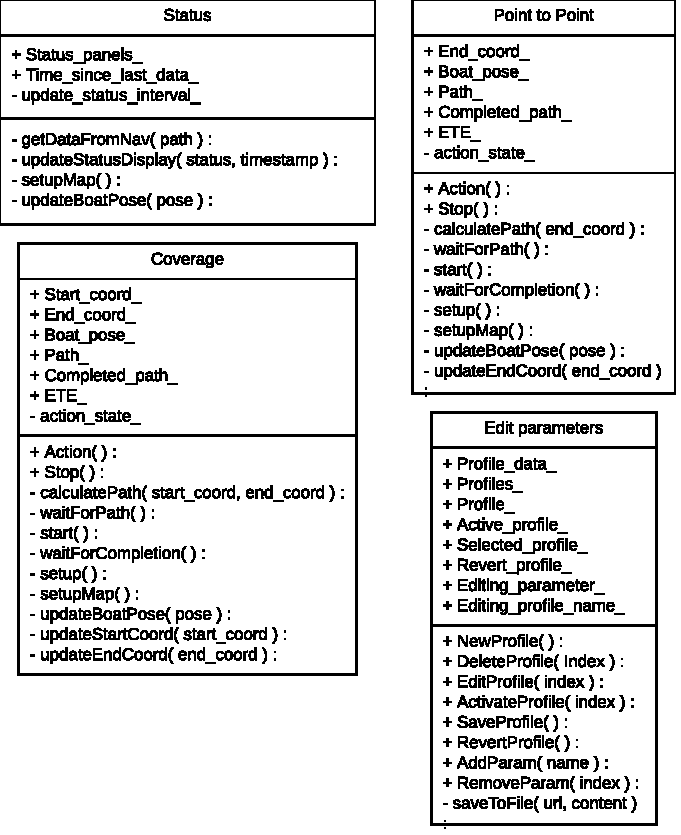
\includegraphics[width=1\linewidth]{Images/Design/User_Interface_overview}
	\caption{An overview of how the functions of the User Interface are structured}
	\label{fig:userinterfaceoverview}
\end{figure}


\subsubsection{Edit parameters}

\paragraph{Public methods:}
These public methods are called on click in the ui.
\begin{adjustwidth}{2.5em}{0pt}\begin{description}
	\item[NewProfile( )] creates a new profile object and appends it to the list of profiles, ie. the member \texttt{Profiles_}. This action then saves the \texttt{Profiles_} to a file.
	\item[DeleteProfile( index )] deletes the profile in the member \texttt{Profiles_} with the designated index. This action then saves the \texttt{Profiles_} to a file.
	\item[EditProfile( index )] displays the profile in the list \texttt{Profiles_} with the index, its profile name, parameters names and their values. \texttt{Revert_profile_} is set to contain the same values.
	\item[ActivateProfile( index )] sets the \texttt{Active_profile_} as the profile in \texttt{Profiles_} with the given index.
	\item[SaveProfile( )]  saves the \texttt{Profiles_} to a file, with the data in the data fields.
	\item[RevertProfile( )] sets \texttt{Profile_} to contain the same values as \texttt{Revert_profile_}.
	\item[AddParam( name )] adds a parameter to the parameter list in \texttt{Profile_}.
	\item[RemoveParam( index )] removes the parameter from the list of parameters in \texttt{Profile_} with the given index.
\end{description}\end{adjustwidth}


\paragraph{Private methods:}
\begin{adjustwidth}{2.5em}{0pt}\begin{description}
	\item[saveToFile( url, content )] sends a \texttt{POST} call to the server at the given url, with the content.
\end{description}\end{adjustwidth}

\paragraph{Public members:}
\begin{adjustwidth}{2.5em}{0pt}\begin{description}
	\item [Profile_data_] contains all the profiles in an encapsulating javascript object.
	\item [Profiles_] contains all the profiles, and resides in the \texttt{Profile_data_} object.
	\item [Profile_] is set to \texttt{Selected_profile_} when \texttt{EditProfile( )} is called.
	\item [Active_profile_] is the active profile.
	\item [Selected_profile_] is the selected profile in \texttt{Profiles_}.
	\item [Revert_profile_] holds the initial configuration of \texttt{Profile_}.
	\item [Editing_profile_] checks whether or not a profile is being edited.
	\item [Editing_profile_name_] checks whether or not a profile name is being edited.
\end{description}\end{adjustwidth}

\subsubsection{Status}

%TODO describe what a status object is in protocols

\paragraph{Private methods:}
\begin{adjustwidth}{2.5em}{0pt}\begin{description}
		\item [getDataFromNav( path )] sends a \texttt{GET} call to the server and gets the file at the path. It must include a status object and a time-stamp object to be valid.
		\item [updateStatusDisplay( status, timestamp )] should dynamically create the user interface elements that correspond to the different statuses in the status object. 
		\item [setupMap( )] sets up the map with appropriate settings.
		\item [updateBoatPose( pose )] updates the position and orientation of the boat on the map.
\end{description}\end{adjustwidth}

\paragraph{Public members:}
\begin{adjustwidth}{2.5em}{0pt}\begin{description}
		\item [Status_panels_] contains the \texttt{HTML} for the different statuses.
		\item [Time_since_last_data] contains how much time has passed since the last time-stamp, as well \texttt{CSS} class for the user interface, which colors the panel according to how much time has passed; blue recent, red dated, orange in between.
\end{description}\end{adjustwidth}


\paragraph{Private members:}
\begin{adjustwidth}{2.5em}{0pt}\begin{description}
		\item [update_status_interval_] is the delay between calls of the \texttt{getDataFromNav( )} function.
\end{description}\end{adjustwidth}


\subsubsection{Point to point}

\paragraph{Public methods:}
\begin{adjustwidth}{2.5em}{0pt}\begin{description}
		\item [Action( )] begins execution of the main task. \texttt{Action( )} first calculates the path, and then runs the path on the subsequent call if the \texttt{Path_} has been calculated. Likewise, the function will not calculate a new \texttt{Path_} before a previous \texttt{Path_} has been completed. 
		\item [Stop( )] stops execution by calling \texttt{saveToFile( )} and resets the state of the \texttt{Action( )} function by resetting \texttt{action_state_}.
\end{description}\end{adjustwidth}

\paragraph{Private methods:}
\begin{adjustwidth}{2.5em}{0pt}\begin{description}
		\item [calculatePath( end_coord )] writes the end_coord and function name to the \texttt{toNav.JSON} file. 
		\item [waitForPath( )] waits for a new \texttt{Path_} to be made available in the \texttt{fromNav.JSON} file, it checks this by way of time-stamps.
		\item [start( )] writes the function name to the \texttt{toNav.JSON} file, in order to tell the system to begin following the calculated \texttt{Path_}.
		\item [waitForCompletion( )] determines if the path has been completed, it does this by checking whether completion percentage is 100\%, coming from the \texttt{fromNav.JSON} file.
		\item [setup( )] sets up the some different variables, could thought of as the constructor.
		\item [setupMap( )] sets up the map with appropriate settings.
		\item [updateBoatPose( pose )] updates the position and orientation of the boat on the map.
		\item [updateEndCoord( end_coord )] updates the \texttt{End_coord_} with a new value.
\end{description}\end{adjustwidth}

%TODO describe polyline

\paragraph{Public members:}
\begin{adjustwidth}{2.5em}{0pt}\begin{description}
		\item [End_coord_] is the end point of the \texttt{Path_}.
		\item [Boat_pose_] is the position and orientation of the boat.
		\item [Path_] is a list of points which is interpreted as a polyline, and is the path that is intended to follow.
		\item[Completed_path_] is a list of points which is interpreted as a polyline, and is the path that the boat actually followed.
		\item[ETE_] contains the estimated time enroute, and the completion percentage, and a \texttt{CSS} class for dynamic styling. 
\end{description}\end{adjustwidth}


\paragraph{Private members:}
\begin{adjustwidth}{2.5em}{0pt}\begin{description}
		\item [action_state_] this is a counter that defines the state of the \texttt{Action( )} function.
\end{description}\end{adjustwidth}

\subsubsection{Coverage}

\paragraph{Public methods:}
\begin{adjustwidth}{2.5em}{0pt}\begin{description}
		\item [Action( )] begins execution of the main task. \texttt{Action( )} first calculates the path, and then runs the path on the subsequent call if the \texttt{Path_} has been calculated. Likewise, the function will not calculate a new \texttt{Path_} before a previous \texttt{Path_} has been completed. 
		\item [Stop( )] stops execution by calling \texttt{saveToFile( )} and resets the state of the \texttt{Action( )} function by resetting \texttt{action_state_}.
\end{description}\end{adjustwidth}

\paragraph{Private methods:}
\begin{adjustwidth}{2.5em}{0pt}\begin{description}
		\item [calculatePath( start_coord, end_coord )] writes the start_coord, end_coord, and function name to the \texttt{toNav.JSON} file. 
		\item [waitForPath( )] waits for a new \texttt{Path_} to be made available in the \texttt{fromNav.JSON} file, it checks this by way of time-stamps.
		\item [start( )] writes the function name to the \texttt{toNav.JSON} file, in order to tell the system to begin following the calculated \texttt{Path_}.
		\item [waitForCompletion( )] determines if the \texttt{Path_} has been completed, it does this by checking whether completion percentage is 100\%, coming from the \texttt{fromNav.JSON} file.
		\item [setup( )] sets up the some different variables, could thought of as the constructor.
		\item [setupMap( )] sets up the map with appropriate settings.
		\item [updateBoatPose( pose )] updates the position and orientation of the boat on the map.
		\item [updateStartCoord( start_coord )] updates the \texttt{Start_coord_} with a new value.
		\item [updateEndCoord( end_coord )] updates the \texttt{End_coord_ }with a new value.
\end{description}\end{adjustwidth}

\paragraph{Public members:}
\begin{adjustwidth}{2.5em}{0pt}\begin{description}
		\item [Start_coord_] is the start point of the coverage rectangle.
		\item [End_coord_] is the end point of the coverage rectangle.
		\item [Boat_pose_] is the position and orientation of the boat.
		\item [Path_] is a list of points which is interpreted as a polyline, and is the path that is intended to follow.
		\item[Completed_path_] is a list of points which is interpreted as a polyline, and is the path that the boat actually followed.
		\item[ETE_] contains the estimated time enroute, and the completion percentage, and a \texttt{CSS} class for dynamic styling. 
\end{description}\end{adjustwidth}


\paragraph{Private members:}
\begin{adjustwidth}{2.5em}{0pt}\begin{description}
		\item [action_state_] this is a counter that defines the state of the \texttt{Action( )} function.
\end{description}\end{adjustwidth}



\subsection{Controller}